\documentclass[a4paper]{article} % papier A4
\usepackage[utf8]{inputenc}      % accents dans le source
\usepackage[T1]{fontenc}         % accents dans le pdf
\usepackage{textcomp}            % symboles complémentaires (euro)
\usepackage[english]{babel}      % titres en français
\usepackage{amsmath}
\usepackage{amsthm}
\usepackage{amssymb}
\usepackage[colorlinks=false]{hyperref} %Apparemment ça sert à rien...
\usepackage{enumerate}
\usepackage{tocloft}             % Pour la table des matières
\usepackage{algorithm}
\usepackage{algorithmic}
\usepackage{pgf}
\usepackage{tikz}
\usepackage{tikz-cd}
\usepackage{rotating}
\usetikzlibrary{matrix,arrows,decorations.pathmorphing}
\usepackage{array}
\usepackage{caption}
\usepackage{graphicx}
% Numérotation des sections, sous-sections, équations, etc.
%\numberwithin{section}{part}
%\numberwithin{equation}{section}

% Maccros pour les commandes de math
\newcommand\nroot[1]{\textit{#1}-ième}
\newcommand\zmodn[1]{\mathbb{Z}/#1\mathbb{Z}}
\newcommand\zmodninv[1]{(\mathbb{Z}/#1\mathbb{Z})^{\times}}
\newcommand\GF[1]{\mathbb{F}_{#1}}
\newcommand\Irr[2]{\textup{min}_{#1}(#2)}
\newcommand\Tr[1]{\textup{Tr}\left(#1\right)}
\newcommand\QQ{\mathbb{Q}}
\newcommand\ZZ{\mathbb{Z}}
\newcommand\NN{\mathbb{N}}
\newcommand\CC{\mathbb{C}}
\newcommand\RR{\mathbb{R}}
\newcommand\EO{\mathcal{O}}
\newcommand\PP[1]{\mathbb{P}^{#1}}
\newcommand\KK{\mathbb{K}}
\newcommand\etmath{\textup{\quad et \quad}}
\newcommand\M[1]{\textup{M}(#1)}
\newcommand\E[1]{\textup{E}(#1)}
\newcommand\I[1]{\textup{I}(#1)}
\newcommand\tO[1]{\widetilde{O}(#1)}
\newcommand\groupgen[1]{\langle{#1}\rangle}
\newcommand\ord[2]{\textup{ord}_{#1}(#2)}
\newcommand{\HRule}{\rule{\linewidth}{0.5mm}}


% Algorithmic en français
\floatname{algorithm}{Algorithme}
\renewcommand{\algorithmicrequire}{\textbf{Entrée :}}
\renewcommand{\algorithmicensure}{\textbf{Sortie :}}
\renewcommand{\algorithmiccomment}[1]{\{#1\}}
\renewcommand{\algorithmicend}{\textbf{fin}}
\renewcommand{\algorithmicif}{\textbf{si}}
\renewcommand{\algorithmicthen}{\textbf{alors}}
\renewcommand{\algorithmicelse}{\textbf{sinon}}
\renewcommand{\algorithmicelsif}{\algorithmicelse\ \algorithmicif}
\renewcommand{\algorithmicendif}{\algorithmicend\ \algorithmicif}
\renewcommand{\algorithmicfor}{\textbf{pour}}
\renewcommand{\algorithmicforall}{\textbf{pour tout}}
\renewcommand{\algorithmicdo}{\textbf{faire}}
\renewcommand{\algorithmicendfor}{\algorithmicend\ \algorithmicfor}
\renewcommand{\algorithmicwhile}{\textbf{tant que}}
\renewcommand{\algorithmicrepeat}{\textbf{répéter}}
\renewcommand{\algorithmicuntil}{\textbf{jusqu'à}}
\renewcommand{\algorithmicreturn}{\textbf{renvoyer}}
\renewcommand{\algorithmicto}{\textbf{à}}

\renewcommand{\listalgorithmname}{Liste des algorithmes}
\renewcommand{\listfigurename}{Liste des figures}



% Éviter l'overlap dans la table des matières pour les sections, sous-sections
% etc.
\setlength{\cftsecnumwidth}{3em}    
\setlength{\cftsubsecnumwidth}{3em} 


\begin{document}
\newtheorem{thm}{Theorem}[section]
\newtheorem{lem}[thm]{Lemma}
\newtheorem{fac}[thm]{Fact}
\newtheorem{cor}[thm]{Corollary}
\newtheorem{prop}[thm]{Proposition}
\newtheorem{conj}[thm]{Conjecture}
\newtheorem*{thmn}{Théorème}
\theoremstyle{definition}
\newtheorem{defn}[thm]{Definition}
\newtheorem{defnp}[thm]{Définition et proposition}
\newtheorem*{ex}{Exemple}
\theoremstyle{remark}
\newtheorem*{rem}{Remarque}
\section{Introduction}
Let $\GF{p}$ be a finite field of characteristic $p\neq2, 3$ and $\GF{p^n}$ be
its extension of degree $n$. We wish to demonstrate the following theorem.

\begin{thm}
\label{conj:gaussellnorm}
Let $m$ be a prime which is not $p$ and $t$ an integer such that : 
\begin{enumerate}[1.]
    \item $|t| < \sqrt{2p}$,
    \item $X^2 - tX + q = (X - \alpha)(X - \beta)\bmod{m}$,
    \item $\zmodninv{m}/\lbrace{\pm1}\rbrace = \groupgen{\alpha}\times S$ for
$S$ a subgroup of $\zmodninv{m}$,
    \item $\ord{m}{\alpha} = n$ and $\ord{m}{\beta}\nmid n$.
\end{enumerate}
Let $E/\GF{p}$ be an ordinary elliptic curve and $t$ be the trace of its
Frobenius map. In that situation, $\GF{p^n}$ is the smallest extension which
contains points $P$ of order $m$ and for all such $P$ in the eigenspace of $\alpha$,
the elliptic periods $\eta_{\alpha}(P)$ form a normal basis on $\GF{p}$.
\end{thm}

More specifically, we wish to demonstrate the fact that said elliptic
periods span $\GF{p^n}$. The proof is actually a secondary result from \cite{MiMoSch}.

\section{Characteristic zero}

Let $E$ be an elliptic curve and $m$ be a prime. We recall that if $m$
is an Elkies prime of $E$ then the characteristic polynomial of the Frobenius
map $\pi$, factors in two linear factor modulo $m$. Consequently, the reduction of $\pi$
to $E[m]$ has two eigenspaces.\par
Let $f_m$ be the division polynomial of order $m$ and $\alpha$ one of the 
eigenvalue of $\pi\bmod{m}$, we note $f_{m,\alpha}$ the generator of one the 
eigenspaces; it is of degree $(m-1)/2$.

\subsection{Preliminaries}
\label{sec:mep}
We will use the notations of \cite{MiMoSch}, let $K$ be the field of definition
of the Deuring lift
\begin{equation}
\widehat{E} : Y^2 = X^3 + \widehat{A}X + \widehat{B}
\end{equation}
of the curve $E$. We introduce the two following extensions : 
\begin{align}
K_m &= K[X]/(\widehat{f}_m(X))\\
L_m &= K_m[Y]/(Y^2 - (X^3 + \widehat{A}X + \widehat{B}))
\end{align}
of degree $m(m-1)/2$ for the former and $2$ for the latter.
We let $\Theta\in K_m$ be the residue class of $X$ modulo $\widehat{f}_m$ and
$\Gamma\in L_m$ be the residue class of $Y$ in $L_m$.\par
Consider $P = (\Theta, \Gamma)$ the generic point of $\widehat{E}(L_m)$, for $a\in 
\zmodninv{m}$ the following action 
\begin{equation}
\rho_a : \Theta \to ([a]\widehat{P})_X
\end{equation}
defines an automorphism of $K_m/K$ and 
\begin{equation}
G = \lbrace{\rho_a : 1 \leq a \leq \dfrac{m-1}{2}}\rbrace
\end{equation}
is a cyclic subgroup of $\textup{Gal}(K_m/K)$ and we let $K_0 = K_m^{G}$ be its
fixed field. The polynomial $\widehat{f}_{m,\lambda}$ factor as 
\begin{equation}
\widehat{f}_{m,\lambda}(T) = \prod_{a=1}^{\tfrac{m-1}{2}}{(T - \rho_a(\Theta))}
\end{equation}
in $K_0[T]$.
Consequently, we have $K_m = K_0[X]/(\widehat{f}_{m,\lambda}(X))$. We can also
define for all $a\in\zmodninv{m}$ the unique polynomial $\widehat{g}_a\in
K_0[X]$ such that $\textup{deg}(\widehat{g}_a) < (m-1)/2$ and $\widehat{g}_a(\Theta) =
\rho_a(\Theta)$, thanks to the fact that the extension is cyclic.

%%%%%%%%%%%%%%%%%%%%%%%%%%%%%%%%%%%%%%%%%%%%%%%%%%%%%%%%%%%%%%%%%%%%%%%%%%%%%%%%%%%%%%%
\iffalse
La situation peut être résumé par le schéma suivant (modulo les notations différentes) : 

\begin{center}
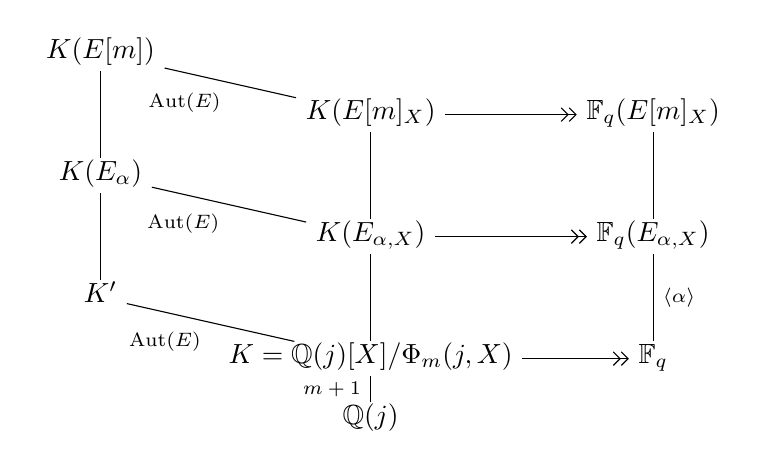
\begin{tikzpicture}
\matrix(m)[matrix of math nodes,
row sep=1em, column sep=2em,
text height=1ex, text depth=0.25ex]
{K(E[m]) & & \\
& K(E[m]_X) & \GF{q}(E[m]_X) \\
K(E_{\alpha}) & & \\
& K(E_{\alpha, X}) & \GF{q}(E_{\alpha, X})\\
K^{\prime} & & \\
& K = \QQ(j)[X]/\Phi_m(j,X) & \GF{q}\\
& \QQ(j) &\\};
\path[-,font=\scriptsize]
(m-7-2) edge node[auto] {$m + 1$} (m-6-2)
(m-6-2) edge node[auto] {} (m-4-2)
(m-4-2) edge node[auto] {} (m-2-2)
(m-6-3) edge node[right] {$\groupgen{\alpha}$} (m-4-3)
(m-4-3) edge node[auto] {} (m-2-3)
(m-5-1) edge node[auto] {} (m-3-1)
(m-3-1) edge node[auto] {} (m-1-1)
(m-6-2) edge node[auto] {Aut($E$)} (m-5-1)
(m-4-2) edge node[auto] {Aut($E$)} (m-3-1)
(m-2-2) edge node[auto] {Aut($E$)} (m-1-1);
\path[->>,font=\scriptsize,>=angle 90]
(m-6-2) edge node[auto] {} (m-6-3)
(m-4-2) edge node[auto] {} (m-4-3)
(m-2-2) edge node[auto] {} (m-2-3);
\end{tikzpicture}
\end{center}
\fi
%%%%%%%%%%%%%%%%%%%%%%%%%%%%%%%%%%%%%%%%%%%%%%%%%%%%%%%%%%%%%%%%%%%%%%%%%%%%%%%%%%%%%%%

\subsection{Elliptic Gaussian period}

Let $c\in\zmodninv{m}$ be a generator. Let $n$ be an odd divisor of $(m-1)/2$
and $n' = (m-1)/(2q)$ its cofactor such that $(n, n') = 1$.
We write $h = c^n$ and $k = c^{n'}$, let $H = \groupgen{h}$ and $K =
\groupgen{k}$; consequently 
\begin{equation}
\zmodninv{m}/\lbrace{\pm1}\rbrace = H \times K
\end{equation}
For $0 \leq i < n$, we define 
\begin{equation}
\widehat{\eta}_i := \sum_{a\in H}{\left([k^ia]\widehat{P}\right)_X} = \sum_{a\in
H}{\rho_a(\rho_{k^i}(\Theta))}
\end{equation}
We notice that $\widehat{\eta}_i = \rho_k^{(i)}(\widehat{\eta}_0)$ for all $ 0 \leq
i < n$; there is a cyclic action
\begin{equation}
\widehat{\eta}_0 \buildrel\rho_k\over\longrightarrow
\widehat{\eta}_1 \buildrel\rho_k\over\longrightarrow \dots 
\buildrel\rho_k\over\longrightarrow \widehat{\eta}_{n-1}
\buildrel\rho_k\over\longrightarrow \widehat{\eta}_0
\end{equation}
from which we can deduce the following result.
\begin{lem}
The polynomial
\begin{equation}
\widehat{M}(T) = \prod_{i = 0}^{n - 1}{(T - \widehat{\eta}_i)}
\end{equation}
is irreducible with coefficients in $\EO(K_0)$. It is the minimal
polynomial of $\widehat{\eta}_0$ over $K_0$.
\end{lem}
\begin{proof}


\end{proof}

\section{Finite field case}

In respect with the notations of \cite{MiMoSch}, we let
\begin{equation}
\mathcal{A}_0 = \GF{p}[X]/(f_{m,\lambda}(X))
\end{equation}
and
\begin{equation}
\mathcal{A} = \GF{p}[X]/(Y^2 - (X^3 + AX + B), f_{m,\lambda}(X)).
\end{equation}
Let $\theta$ and $\gamma$ be the residue class of $X$ and $Y$ in $\mathcal{A}$.
We write $P = (\theta, \gamma)$ the generic point in the eigenspace of $\alpha$. 
Like in section \ref{sec:mep}, for $a\zmodninv{m}$ we define the unique 
polynomials $g_a$ of degree inferior to $(m-1)/2$ such that $g_a(\theta) = 
([a]P)_X \in\mathcal{A}$.

\begin{fac}
If $m$ is an Elkies prime for $E/\GF{p}$, then there exists a prime $\mathfrak{p}$ of
$\EO(K_0)$ above $p$ such that 
$\widehat{f}_{m,\lambda}=f_{m,\lambda}\bmod\mathfrak{p}$, \emph{i.e.} the 
polynomial $\widehat{f}_{m,\lambda}$ is a cyclic lift of $f_{m,\lambda}$; in a 
similar way, the $\widehat{g_a}$ are cyclic lifts of $g_a$ for all 
$a\in\zmodninv{m}$.
\end{fac}
\begin{proof}
TODO
\end{proof}
Then by the definition of $g_a$, we can write 
\begin{equation}
f_{m,\lambda}(Z) = \prod_{a=1}^{\tfrac{l-1}{2}}{(Z - g_a(\theta))}.
\end{equation}
For $0 \leq i < q$, we define 
\begin{equation}
\eta_i = \sum_{a\in H}{g_a(g_{k^i}(\theta))}
\end{equation}
in particular $\eta_i = \widehat{\eta}_i \bmod \mathfrak{p}$. We remind that for
odd $m\geq3$, the discriminant of $f_m(X)$ satisfies the following relation
\begin{equation}
\textup{Disc}(f_m) = (-1)^{(m-1)/2}m^{(m^2 - 3)/2}(-\Delta)^{(m^2 - 1)(m^2 -
3)/24}
\end{equation}
where $\Delta = \Delta(E)$ is the discriminant of $E$. Therefore the roots of
$f_m(X)$, and $f_{m,\lambda}(X)$, are distinct. Which, in turn,
implies that for $i\neq j$, we have $\eta_i\neq\eta_j$, because otherwise we 
could find a linear relation between the roots of $f_{m,\lambda}$. From there, 
we can conclude that the reduction of $\widehat{M}(T)$ is separated.\par
Finally, if we write $M(T)\in\GF{p}[T]$ the minimal polynomial of
$\eta_0\in\mathcal{A}_0$ and note that $M(T) = \widehat{M}(T)\bmod
\mathfrak{p}$, we get that the degree of $M(T)$ is $n$.

\section{Result}

Now that we have everything we need, we can finish the proof of the
theorem.
Let $E/\GF{p}$ be an elliptic curve and $m$ an Elkies prime for $E$. We also write
$\alpha$ and $\beta$ the two eigenvalues of the Frobenius of $E$.\par
We recall the hypothesis. One of the eigenvalue, say $\alpha$, must be of order $n$
in $\zmodninv{m}$ and $\beta$ must be of order not dividing by $n$. This means
that $n$ is an odd divisor of $\varphi(m) = m-1$ and is prime to $(m-1)/n$; it 
is also prime to $(m-1)/2n$.\par
Let $P$ by a point in the eigenspace of $\alpha$. We then pick a generator
$c\in\zmodninv{m}$ such that $\alpha = c^{n'}$ where $n' = (m-1)/2n$, so we can
have the following situation
\begin{equation}
\zmodninv{m}/\lbrace{\pm1\rbrace} = \groupgen{\alpha}\times H
\end{equation}
where $H = \groupgen{h}$ and $h = c^n$.\par
From the previous section, we can deduce that the minimal polynomial of
\begin{equation}
\eta_{\alpha}(P) := \eta_0 = \sum_{a\in H}{g_a(\theta)} = \sum_{a\in
H}{([a]P)_X}
\end{equation}
is $M(T)$ which is of degree $n$. As this stand for any point $P$ of the
eigenspace of $\alpha$, we have therefore proved the point we wanted to.

\begin{thebibliography}{LC}

\bibitem{MiMoSch} \emph{Computing the Eigenvalue in the Schoof-Elkies-Atkin
Algorithm using Abelian Lifts}, P. Mih\u{a}ilescu, F. Morain \&
É. Schost, 2007, url :
\url{http://hal.inria.fr/LIX/inria-00130142/en/}

\end{thebibliography}


\end{document}
